\documentclass[final]{beamer}
%% Possible paper sizes: a0, a0b, a1, a2, a3, a4.
%% Possible orientations: portrait, landscape
%% Font sizes can be changed using the scale option.
\usepackage[size=a1,orientation=portrait,scale=1.1]{beamerposter}

\usetheme{gemini}
\usecolortheme{seagull}
\useinnertheme{rectangles}

% ====================
% Packages
% ====================

\usepackage[utf8]{inputenc}
\usepackage{graphicx}
\usepackage{booktabs}
\usepackage{tikz}
\usepackage{pgfplots}
\usepackage{svg}
\usepackage{amsmath,amssymb,amsfonts}
\usepackage{multicol}
\usepackage{placeins}
\usepackage[noend]{algpseudocode}
\usepackage{amsmath}
 

% ====================
% Lengths
% ====================

% If you have N columns, choose \sepwidth and \colwidth such that
% (N+1)*\sepwidth + N*\colwidth = \paperwidth
\newlength{\sepwidth}
\newlength{\colwidth}
\setlength{\sepwidth}{0.03\paperwidth}
\setlength{\colwidth}{0.45\paperwidth}

\newcommand{\separatorcolumn}{\begin{column}{\sepwidth}\end{column}}

% ====================
% Logo (optional)
% ====================

% LaTeX logo taken from https://commons.wikimedia.org/wiki/File:LaTeX_logo.svg
% use this to include logos on the left and/or right side of the header:
\logoleft{\includegraphics[height=6.6cm]{logo/iub_cse.png}}
\logoright{\includegraphics[height=6.6cm]{logo/iub_logo.png}}

% ====================
% Footer (optional)
% ====================

\footercontent{
	\insertdate \hfill
	Algorithm Project \hfill
	CSE211: Algorithms Lab
    % \href{mailto:myemail@exampl.com}{\texttt{myemail@example.com}}
}
% (can be left out to remove footer)

% ====================
% My own customization
% - BibLaTeX
% - Boxes with tcolorbox
% - User-defined commands
% ====================
% ====================
% BibLaTeX
% ====================

\usepackage[backend=biber,
	bibstyle=authoryear,
	citestyle=authoryear,
	style=authoryear,
	maxcitenames=2,
	maxbibnames=20, % limit the length of list of names (authors/editors/etc.)
	sorting=ydnt, % sort references by year (descending), name, title
	dashed=false, % show authors instead of dash in publications having the same authors
	giveninits=true % render authors' given name initials and not the full given names
]{biblatex}
%% Biblatex with Beamer bibliography icons
\setbeamertemplate{bibliography item}{%
	\ifboolexpr{ test {\ifentrytype{book}} or test {\ifentrytype{mvbook}}
		or test {\ifentrytype{collection}} or test {\ifentrytype{mvcollection}}
		or test {\ifentrytype{reference}} or test {\ifentrytype{mvreference}} }
	{\setbeamertemplate{bibliography item}[book]}
	{\ifentrytype{online}
		{\setbeamertemplate{bibliography item}[online]}
		{\setbeamertemplate{bibliography item}[article]}}%
	\usebeamertemplate{bibliography item}}
\defbibenvironment{bibliography}
{\list{}
	{\settowidth{\labelwidth}{\usebeamertemplate{bibliography item}}%
		\setlength{\leftmargin}{\labelwidth}%
		\setlength{\labelsep}{\biblabelsep}%
		\addtolength{\leftmargin}{\labelsep}%
		\setlength{\itemsep}{\bibitemsep}%
		\setlength{\parsep}{\bibparsep}}}
{\endlist}
{\item}
%% Redefine \refname
\renewcommand{\bibname}{References}
%% Redefine \parencite to use square brackets instead of braces
\DeclareCiteCommand{\parencite}
{\usebibmacro{prenote}}
{\usebibmacro{citeindex}%
	\printtext[bibhyperref]{[\usebibmacro{cite}]}}
{\multicitedelim}
{\usebibmacro{postnote}}
%% Highlight author names using Beamer data annotation
%% Usage: add a new line `author+an = {<author-order>=highlight}` to an entry
%% For example: author+an = {3=highlight} => highlight the 3rd author name
\AtBeginBibliography{
	\renewcommand*{\mkbibnamegiven}[1]{%
		\ifitemannotation{highlight}
		{\textbf{#1}}
		{#1}%
	}
	
	\renewcommand*{\mkbibnamefamily}[1]{%
		\ifitemannotation{highlight}
		{\textbf{#1}}
		{#1}%
	}
}

% ====================
% Boxes with tcolorbox
% ====================
\usepackage[most]{tcolorbox}

%%% Beamer colors in boxes

\newcommand{\beamercolorsinboxes}[1]{
	\setbeamercolor{itemize item}{fg=#1!75!black}
	\setbeamercolor{itemize/enumerate body}{fg=#1!65!white}
	\setbeamercolor{itemize/enumerate subbody}{fg=#1!65!white}
	\setbeamercolor{item projected}{fg=white, bg=#1!75!black}
}

%%% Highlight Oval Box
\newtcbox{\xmybox}[1][red]{on line,
	arc=7pt,colback=#1!10!white,colframe=#1!50!black,
	before upper={\rule[-3pt]{0pt}{10pt}},boxrule=1pt,
	boxsep=0pt,left=6pt,right=6pt,top=2pt,bottom=2pt}
%%% Box for stating problems
%%%%%%%%
%Usage: (similar for infobox)
%	\begin{defbox}{title}
	%		contents
	%	\end{defbox}
%%%%%%%%
\newtcolorbox{defbox}[1]{%
	enhanced,
	attach boxed title to top 	left={xshift=5mm,yshift=-5mm,yshifttext=-5mm},
	colback=cyan!5!white,
	colframe=cyan!75!black,
	coltitle=cyan!80!black,
%	left=0mm,right=0mm,top=2mm,bottom=0mm,
	title={#1},
	fonttitle=\bfseries\large, fontupper=\color{cyan!65!white},
	boxed title style={colback=cyan!5!white,colframe=cyan!75!black},
	before upper={
		\beamercolorsinboxes{cyan}
	}
}%
%%% Box for announcement
\newtcolorbox{infobox}[1]{%
	enhanced,
	attach boxed title to top 	left={xshift=5mm,yshift=-5mm,yshifttext=-5mm},
	colback=yellow,
	colframe=red!75!black,
	coltitle=red!75!black,
%	left=0mm,right=0mm,top=2mm,bottom=0mm,
	title={#1},
	fonttitle=\bfseries\large, fontupper=\color{red!65!white},
	boxed title style={colback=yellow,colframe=red!75!black},
	before upper={
		\beamercolorsinboxes{red}
	}
}%
%%% Box for example
\newtcolorbox{exabox}[1]{%
	enhanced,
	attach boxed title to top 	left={xshift=5mm,yshift=-5mm,yshifttext=-5mm},
	colframe=brown!75!black,colback=brown!5!white,coltitle=brown!50!brown!75!black,
%	left=0mm,right=0mm,top=2mm,bottom=0mm,
	title={#1},
	fonttitle=\bfseries\large, fontupper=\color{brown!65!white},
	boxed title style={colback=brown!5!white,coltitle=brown!50!brown!75!black},
	before upper={
		\beamercolorsinboxes{brown}
	}
}%
%%% Theorem Box
%%%%%%%%
%Usage: (similar for conjecture, lemma, etc.)
%	\begin{thm}{title}{nameref}
	%		contents
	%	\end{thm}
% Use \ref{thm:nameref} to refer to the theorem
%%%%%%%%
%%%% Use \newtcbtheorem[number within=section]{thm} to number within each section
\newtcbtheorem[]{thm}%
{Theorem}{attach boxed title to top 	left={xshift=5mm,yshift=-5mm,yshifttext=-5mm},
	enhanced jigsaw,
	%	top=2mm,bottom=0mm,left=0mm,right=0mm,
	fonttitle=\bfseries\large,fontupper=\itshape\color{blue!65!white},
	colframe=blue!75!black,colback=blue!5!white,coltitle=blue!50!blue!75!black,
	boxed title style={colback=blue!5!white,coltitle=blue!50!blue!75!black},
	before upper={
		\beamercolorsinboxes{blue}
	}
}{thm}%
%%% Proposition Box
\newtcbtheorem[use counter from=thm]{prop}%
{Proposition}{attach boxed title to top 	left={xshift=5mm,yshift=-5mm,yshifttext=-5mm},
	enhanced jigsaw,
	%	top=2mm,bottom=0mm,left=0mm,right=0mm,
	fonttitle=\bfseries\large,fontupper=\itshape,
	colframe=gray!75!black,colback=gray!5!white,coltitle=gray!50!gray!75!black,
	boxed title style={colback=gray!5!white,coltitle=gray!50!gray!75!black},
	before upper={
		\beamercolorsinboxes{gray}
	}
}{prop}%
%%% Conjecture Box
\newtcbtheorem[use counter from=thm]{conj}%
{Conjecture}{attach boxed title to top 	left={xshift=5mm,yshift=-5mm,yshifttext=-5mm},
	enhanced jigsaw,
	%	top=2mm,bottom=0mm,left=0mm,right=0mm,
	fonttitle=\bfseries\large,fontupper=\slshape,
	colframe=orange!75!black,colback=orange!5!white,coltitle=orange!50!orange!75!black,
	boxed title style={colback=orange!5!white,coltitle=orange!50!orange!75!black},
	before upper={
		\beamercolorsinboxes{orange}
	}
}{conj}%
%%% Lemma Box
\newtcbtheorem[use counter from=thm]{lem}%
{Lemma}{attach boxed title to top 	left={xshift=5mm,yshift=-5mm,yshifttext=-5mm},
	enhanced jigsaw,
	%	top=2mm,bottom=0mm,left=0mm,right=0mm,
	fonttitle=\bfseries\large,fontupper=\itshape,
	colframe=green!75!black,colback=green!5!white,coltitle=green!50!green!75!black,
	boxed title style={colback=green!5!white,coltitle=green!50!green!75!black},
	before upper={
		\beamercolorsinboxes{green}
	}
}{lem}%
%%% Claim Box
\newtcbtheorem[use counter from=thm]{clm}%
{Claim}{attach boxed title to top 	left={xshift=5mm,yshift=-5mm,yshifttext=-5mm},
	enhanced jigsaw,
	%	top=2mm,bottom=0mm,left=0mm,right=0mm,
	fonttitle=\bfseries\large,fontupper=\itshape,
	colframe=pink!75!black,colback=pink!5!white,coltitle=pink!50!pink!75!black,
	boxed title style={colback=pink!5!white,coltitle=pink!50!pink!75!black},
	before upper={
		\beamercolorsinboxes{pink}
	}
}{clm}%

%Configs

\def\inst#1{\unskip$^{#1}$}
\def\orcidID#1{\unskip$^{[#1]}$} % added MR 2018-03-10
\def\fnmsep{\unskip$^,$}
\def\email#1{{\tt#1}}



%% Reference Sources
\addbibresource{refs.bib}
\renewcommand{\pgfuseimage}[1]{\includegraphics[scale=2.0]{#1}}

\pgfplotsset{compat=1.18}



\title{Multi-way Chaining}

\author
{
    Lamisha Shajnin \inst{1} \and
    Md. Raihan Hossain  \inst{2} \and
    Mustaqueem Alam\inst{3} \and 
    Refaya Aftarin \inst{4} 
    Supprio Ghosh Nil \inst{5}    
}

% \institute[shortinst]{\inst{1} Independent University Bangladesh \samelineand \inst{2} Another Institute}

\institute{Department of Computer Science and Engineering\\Independent University, Bangladesh\\Dhaka, Bangladesh.\\
\email{\{$^{1}$2220325},{$^{2}$2220750},{$^{3}$2220769},{$^{4}$2221056},{$^{5}$2221077}@iub.edu.bd}
%\url{http://www.springer.com/gp/computer-science/lncs} 
 }
\date{Autumn, 2022}

\begin{document}
	
\begin{frame}[t]
	
	\begin{columns}[t]
	
	\begin{column}{2\colwidth+\sepwidth}	\begin{exampleblock}{Abstract}
	\justifying{

    A multi-way chain is such an algorithm which allows efficient storage and retrieval of large amounts of data. This algorithm is based on the concept of a chain in which every link in the chain contains a fixed number of
elements known as a block. The data is divided into multiple blocks where each block is linked to the very next block in the chain. The blocks are then stored in the memory and can be accessed using pointers.\\
The main function of this algorithm is its ability to efficiently store and retrieve large amounts of data when the data is too large and to allow efficient reversals of the data structures as each block contains pointers to the next block in the chain. However, this algorithm can be complex to implement sometimes, as it requires proper management of the block sizes and the pointers between the blocks.
         
    }
	\end{exampleblock}
	\end{column}

	\end{columns}

	\begin{columns}[t]
		\separatorcolumn
		
		\begin{column}{\colwidth}
			
			\begin{block}{Introduction}
			\justifying
            \textbf{What is Multi-way Chaining?}\\
The algorithm, multi-way chaining is used to handle collisions in a hash table as when a collision occurs, the reason is that the function finds two or more keys at the same index.  This kind of an algorithm can be used to solve many problems related to  fast accessing the data item, such as Symbol table management, Data compression, Database indexing & Network packet routing. In simple words, any problem which requires storing, retrieving, or processing vast amount of data can benefit from the multi-way chaining algorithm.\\
The multi-way chaining algorithm was first proposed by the computer scientist and mathematician, \textbf{Donald Knuth}.  Knuth introduced the algorithm in his book \textbf{"The Art of Computer Programming"} as a method for resolving collisions in hash tables.\\
It can handle an arbitrary number of collisions at a single index in the hash table. It uses memory efficiently. It delivers good performance for small and medium-sized data sets.\\
It has poor cache locality since the linked lists are not stored in contiguous memory locations. It needs a good hash function. It becomes high memory overhead, especially for large data sets\\
\textbf{Paradigm:} Depending on the specific requirements and constraints of the problem, the multi-way chains algorithm can be implemented using various programming paradigms. \\ 
\textbf{Graph-based paradigm:}\\
The traversal and manipulation of the graph using standard graph algorithms is efficient. It can easily handle large and complex data-sets. It provides a visual representation of the data-set.\\
It requires a significant amount of memory and processing power and may not be suitable for problems that involve complex data structures or non-linear relationships.\\
\textbf{Greedy algorithmic paradigm:}\\
It is simple and easy to implement and efficient for those problems which involve finding a single optimal solution.\\
It might not always lead the the desired solution. It is sensitive to the initial conditions and may not be robust to changes in the data-set or problem constraints.
\\
\textbf{Time complexity analysis:}\\ 
The time complexity of the multi-way chain algorithm is more dependent on specific implementations and distribution of the search keys present in the linked list.\\
\textbf{Average case:}  O(n/2) or  O(n)
\textbf{worst case:} O(n)
\textbf{best case:} O(1)
                    

				
			\end{block}
			\begin{block}{Rationale for the Algorithm's Selection}
			\justifying
            The algorithm we are discussing is multi-way chaining. In this algorithm, when a
collision happens, it gets sorted out by the use of a linked list. Here each slot of the
hash table contains a linked list.\\
Let’s say we want to create a hash table to store the information of the employees working in a company. The system desires to store their designated unique ID number, name, department, address, and salary. In this case, there will be a large number of employees, which will result in a huge
amount of data. So, if we can assign each of set of data of the respective employee to a certain slot in the hash table, then the data will get arranged. But as there are too many
employees, there will be a great chance that multiple ID numbers will attain the same slot for which, a collision will occur.\\
So, to solve this collision, we will use the multi-way chaining algorithm. For this algorithm, when multiple ID numbers will point at the same slot, the data will get
inserted into the built-in linked list where it will find the last empty slot of the list.\\
            
			\end{block}
			
			\begin{alertblock}{Methodology}   
                \begin{multicols}{2}
                 To solve the problem discussed previously, the algorithm will work as described below:\\ 
Firstly, we will have a simple hash function where a modulus of the ID number and the size of the hash table would occur, and we will get our result, which will be the hash value\\ 
\textbf{Hash (ID) = ID \% table.size()~}\\
So, in this case, if our table has 10 slots, if the ID number of our employee is 53, the hash will be 3 which indicates the 3rd slot.\\ 
Now, if we add another ID number of about 43, the hash result will be 3. Hence, we will see a collision there. Now, instead of over-writing, we will use the multi-chaining method for which the data will be added to a linked list at the 3 rd slot.
Now, if we have to add any more ID information here, we can easily do so. • For this, when any ID number will be searched in the system to get all the information after the hash function is called again, the pointer will go to the designated slot and will go through the entire linked list
to find the match.
\columnbreak
\begin{figure}
    \centering
    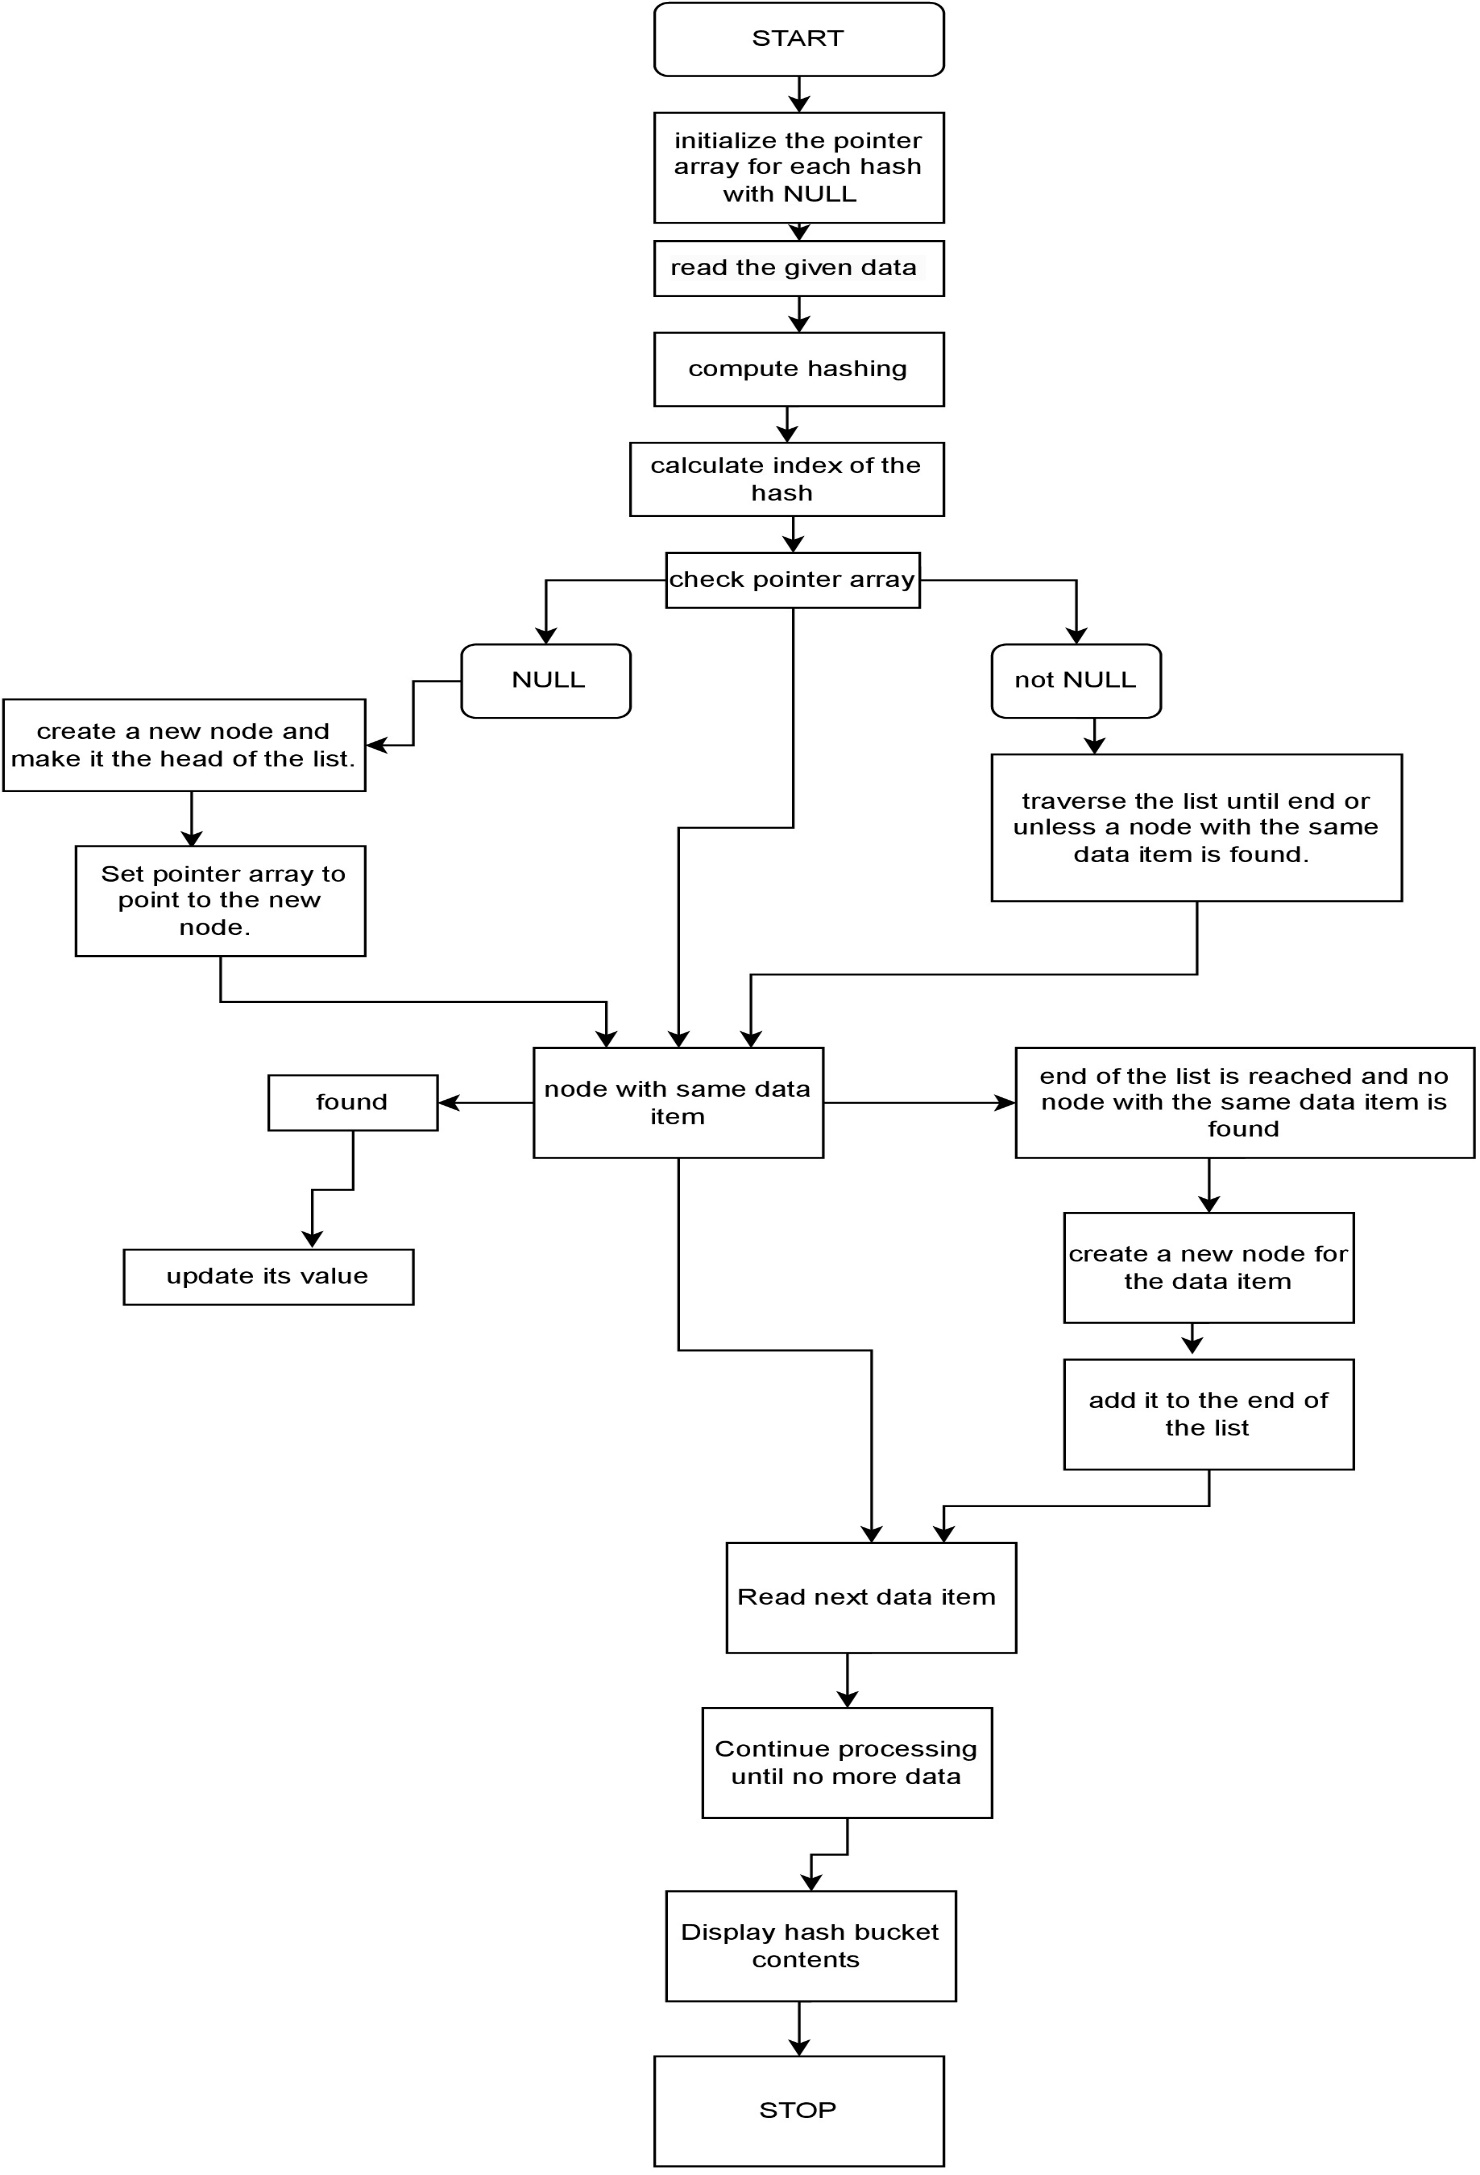
\includegraphics[width=12cm,height=20cm]{image3.jpeg}
\end{figure}
        \end{multicols}
	\end{alertblock}
        
			
		\end{column}
	
		\separatorcolumn
		
		\begin{column}{\colwidth}
			
			\begin{alertblock}{Substitute Use of the Algorithm}{}
            
            While multilevel hashing is primarily used to improve the performance of hash tables, it can also be used in other applications. So here are the substitute uses of multi-way chains hashing:\\
1. For creating a secure password storage system by hashing passwords using multiple hash functions and storing the resulting hashes in a database.\\
2. Comparing hashed user input to the hashes stored in the database to authenticate a user's password during login.\\
3. Improving the efficiency and security of various applications in computer science and beyond by using multilevel hashing.\\
4. Improving the performance of hash tables by using multiple hash functions in a cascading fashion to map keys to a sequence of slots.\\
5. Partitioning large data sets across multiple servers and using multilevel hashing to store and retrieve data efficiently in a distributed computing environment.\\
6. It can be used in content-addressable memory (CAM) systems, where the data is searched based on the content rather than an address.\\
7. Multilevel hashing can be used in DNA sequencing to efficiently search for matching sequences in a large database of genetic data. In this context, multilevel hashing can improve the search speed and reduce the storage requirements of the database.\\

            
			\end{alertblock}
   
   		\begin{alertblock}{Alternative Solution}
			\justifying
             The multi-way chain algorithm is one of the most efficient algorithms for finding the longest common sub-sequence of multiple sequences. However, there are other algorithms that could be used, depending on the specific requirements of the problem. For example, in case the arrangements are very long, at that point a divide-and-conquer approach such as the Hirschberg's calculation might be more proficient.
On the other hand, if the sequences are short, then a dynamic programming approach may be more
efficient.\\
In general, it is always worth considering alternative algorithms when trying to optimize
performance. It is important to carefully evaluate the trade-offs between different algorithms in terms of
their time complexity, space complexity, and other factors relevant to the specific problem being solved.\\
Here are some general tips for improving system performance:\\
\textbf{Optimize for speed and efficiency:} Multi way chain algorithms can involve complex computations and
large data-sets. To improve performance, consider optimizing the algorithm for speed and efficiency. This could involve techniques like parallel processing, caching, and optimizing memory usage.\\
\textbf{Expand the scope:} Multi way chain algorithms can be applied to a wide range of use cases, so consider
expanding the scope of the algorithm to address additional problems. This could involve incorporating
new data sources or developing new analytical techniques.\\
\textbf{Increase accuracy:} Depending on the specific use case, improving the accuracy of the algorithm could be a key priority. This could involve refining the algorithm itself or improving the quality of the data it uses.\\
\textbf{Improve user experience:}  Finally, consider ways to improve the user experience of the system. This could involve designing a more intuitive user interface or providing additional tools and resources to help
users understand and interpret the results of the algorithm.
These are just a few general tips for improving system performance.


             
			\end{alertblock}
   
			\begin{alertblock}{Conclusion}
			\justifying
             In conclusion, the multi-way chaining is a wonderful algorithm to manage the collisions in hash table. This algorithm is used to store a huge amount of data where many information's of the data-set can be matched with each other and face a collision in hash tables.\\
The multi-way chaining algorithm is mainly implemented by graph based paradigm which represents the data set as a acyclic directed graph. While it is working firstly it initializes the pointer array for each hash and then calculate index of calculated hash of the given data then it checks the pointer array. If the array is null then it set pointer array to a new created node. Also when the pointer array is not null then it traverses the list until it finds any node with same data. If the node with same data is found then it updates the value and if there is no node with same data then it creates a new node for the data item by adding it to the end. After all these processes it reads the next data and continues the procedure until there is no more data. Finally it displays the hash bucket.\\
So the multi-way chaining would be the best solution when someone work with a huge data set to manage the data in a efficient way.

             
			\end{alertblock}
		\end{column}
		
		\separatorcolumn
	\end{columns}
    \end{frame}
\end{document}